The timing properties, and other features measured by the timing model, for
over 2000 pulsars observed can be accessed via the Australia Telescope National
Facility (ATNF) pulsar catalogue \citep{ATNF}.  We can categorise the
population by their measured values of period $P$ and the period derivative
$\Pdot$. This is done by plotting them in a so-called $P - \Pdot$ diagram, as
shown in Fig.~\ref{fig: Period_PeriodDot}.  The various categories to which
each pulsar can be assigned have been marked in this plot and we now discuss
their features.

\begin{figure}[htb]
\centering
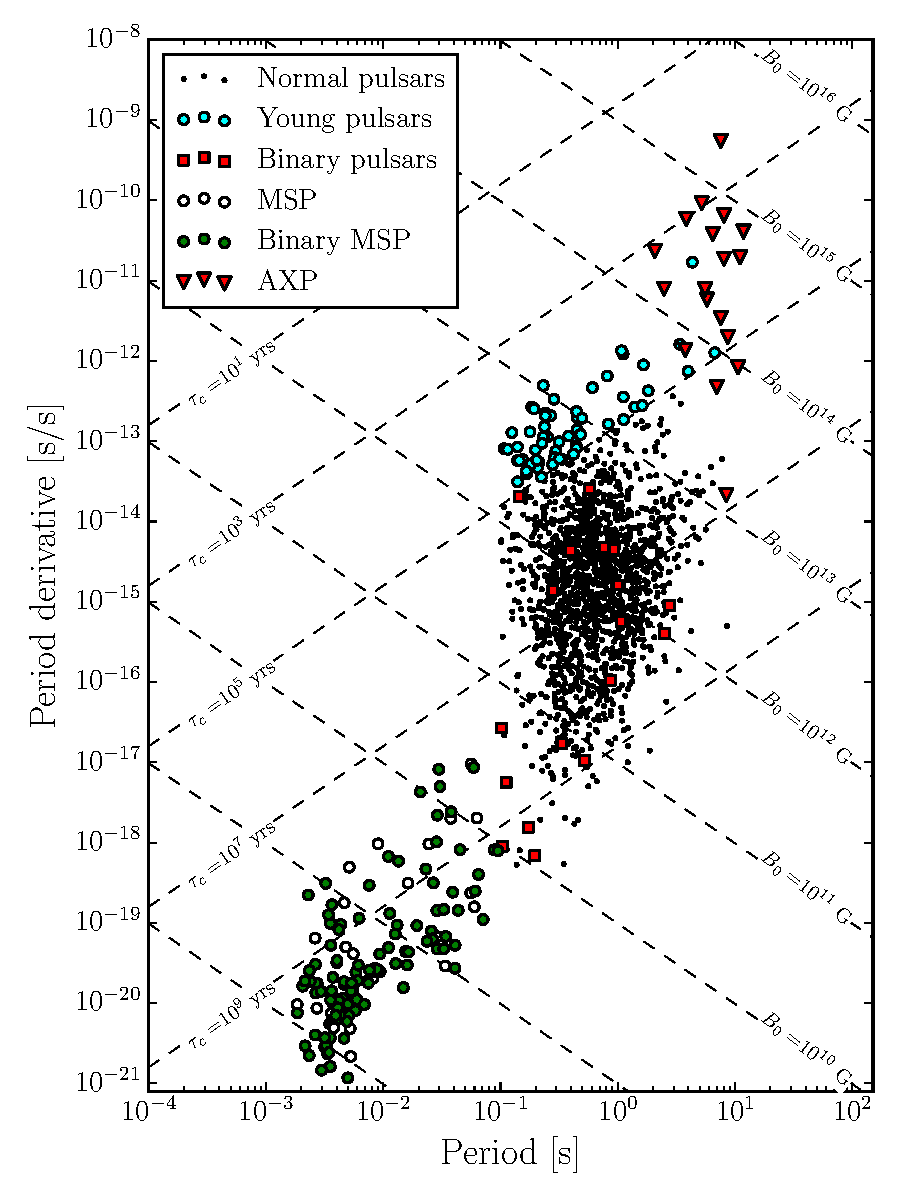
\includegraphics[width=0.8\textwidth]{Period_PeriodDot} 
\caption{Period -
Period derivative diagram using data taken from the ATNF pulsar catalogue
\citep{ATNF}. Dashed lines show inferred magnetic fields and characteristic
ages as described in Sec.~\ref{sec: rotation powered pulsars}}
\label{fig: Period_PeriodDot}
\end{figure}

The majority of pulsars (referred to as the `normal' pulsars) are found
\emph{isolated} without a binary companion and have typical periods of
$P=10^{-1}-10^{1}$~s. These can be described as \emph{rotation powered}
pulsars, since the electromagnetic (EM) radiation is powered by the loss of
rotational energy. As described later in Sec.~\ref{sec: rotation powered
pulsars}, estimates can be made of their characteristic age, $\tauAge$, and
surface magnetic field strength, $B_{0}$, based on a dipole spin-down model.
Constant lines of these quantities are plotted in Fig.~\ref{fig:
Period_PeriodDot}. Of the normal pulsars, we can choose to identify the young
pulsars as those for which $\tauAge<10^{5}$~yrs. Some of these, such as the
Crab and Vela pulsars, can be directly associated with their supernova remnant
from which they were formed \citep{Kaspi1996}.

A second smaller population of isolated rotation powered pulsars exists with
$P<10^{-1}$~s. These are known as the \emph{millisecond pulsars} (MSPs). This
special class of pulsars are believed to start their life as normal pulsars,
but are then spun-up through accretion from a normal star. In support of this
hypothesis, the majority of MSPs in Fig.~\ref{fig: Period_PeriodDot} have a
binary companion \citep{wijnands1998millisecond}. Additionaly, we see so-called
low-mass X-ray binary systems (LMXBs) which are systems where a neutron star in
a binary accretes matter from its companion; the infalling matter releases
gravitational potential energy in the form of X-rays \citep{lewin1997x}. It is
thought that these LMXBs are the progenitors of the MSPs, recent results of
`transitional systems' (see for example \citep{archibald2009radio}) which
switch between the two seem to confirm this.

We include one final class of neutron stars, \emph{magnetars}, thought to have
large magnetic fields of $B\gtrsim 5\times10^{13}$~G. These are in fact
observed from two channels which we will now describe. Some pulsars are
observed to emit X-ray radiation; usually this is powered by the accretion of
matter from a binary companion, but this mechanism does not apply to isolated
stars, subsequently isolated stars observed in the X-ray band where named
\emph{anomalous X-ray pulsars} (AXPs). It was shown by
\citet{duncan1996magnetars} that AXPs are magnetars where the emmission is
powered by the decay of the strong magnetic field.  At the same time,
astronomers found a class of objects emmitting irregular bursts of
$\gamma$-rays or X-rays which they named the \emph{soft $\gamma$-ray repeaters}
(SGRs). As discussed in \citet{kouveliotou2003magnetars} these are now
understood to be magnetars which undergo rearrangement of their magnetic
fields. The two individual observations where unified by observation of X-ray
bursts from AXPs by \citet{Gavriil2002}. In Fig.~\ref{fig: Period_PeriodDot} we
label observations from both these sources as magnetars.
